\documentclass[10pt]{article}

%%%%%%%%%%%%%%%%%%%%%%%%%%%%%%%%%%%%%%%%%%%%%%%%%%%%%%%%%%%%%%%%%%%%%%%%%%%%%%%%
% LaTeX Imports
%%%%%%%%%%%%%%%%%%%%%%%%%%%%%%%%%%%%%%%%%%%%%%%%%%%%%%%%%%%%%%%%%%%%%%%%%%%%%%%%
\usepackage{amsfonts}                                                   % Math fonts
\usepackage{amsmath}                                                    % Math formatting
\usepackage{amssymb}                                                    % Math formatting
\usepackage{amsthm}                                                     % Math Theorems
\usepackage{arydshln}                                                   % Dashed hlines
\usepackage{attachfile}                                                 % AttachFiles
\usepackage{cancel}                                                     % Cancelled math
\usepackage{caption}                                                    % Figure captioning
\usepackage{color}                                                      % Nice Colors
\input{./lib/dragon.inp}                                                % Tikz dragon curve
\usepackage[ampersand]{easylist}                                        % Easy lists
\usepackage{fancyhdr}                                                   % Fancy Header
\usepackage[T1]{fontenc}                                                % Specific font-encoding
%\usepackage[margin=1in, marginparwidth=2cm, marginparsep=2cm]{geometry} % Margins
\usepackage{graphicx}                                                   % Include images
\usepackage{hyperref}                                                   % Referencing
\usepackage[none]{hyphenat}                                             % Don't allow hyphenation
\usepackage{lipsum}                                                     % Lorem Ipsum Dummy Text
\usepackage{listings}                                                   % Code display
\usepackage{marginnote}                                                 % Notes in the margin
\usepackage{microtype}                                                  % Niceness
\usepackage{lib/minted}                                                 % Code display
\usepackage{./lib/mlptikz}                                              % Tikz mlp
\usepackage{multirow}                                                   % Multirow tables
\usepackage{pdfpages}                                                   % Include pdfs
\usepackage{pgfplots}                                                   % Create Pictures
\usepackage{rotating}                                                   % Figure rotation
\usepackage{setspace}                                                   % Allow double spacing
\usepackage{subcaption}                                                 % Figure captioning
\usepackage{tikz}                                                       % Create Pictures
\usepackage{tocloft}                                                    % List of Equations
%%%%%%%%%%%%%%%%%%%%%%%%%%%%%%%%%%%%%%%%%%%%%%%%%%%%%%%%%%%%%%%%%%%%%%%%%%%%%%%%
% Package Setup
%%%%%%%%%%%%%%%%%%%%%%%%%%%%%%%%%%%%%%%%%%%%%%%%%%%%%%%%%%%%%%%%%%%%%%%%%%%%%%%%
\hypersetup{%                                                           % Setup linking
    colorlinks=true,
    linkcolor=black,
    citecolor=black,
    filecolor=black,
    urlcolor=black,
}
\RequirePackage[l2tabu, orthodox]{nag}                                  % Nag about bad syntax
\renewcommand*\thesection{\arabic{section}}                             % Reset numbering
\renewcommand{\theFancyVerbLine}{{\arabic{FancyVerbLine}}}              % Needed for code display
\renewcommand{\footrulewidth}{0.4pt}                                    % Footer hline
\setcounter{secnumdepth}{3}                                             % Include subsubsections in numbering
\setcounter{tocdepth}{3}                                                % Include subsubsections in toc
%%%%%%%%%%%%%%%%%%%%%%%%%%%%%%%%%%%%%%%%%%%%%%%%%%%%%%%%%%%%%%%%%%%%%%%%%%%%%%%%
% Custom commands
%%%%%%%%%%%%%%%%%%%%%%%%%%%%%%%%%%%%%%%%%%%%%%%%%%%%%%%%%%%%%%%%%%%%%%%%%%%%%%%%
\newcommand{\nvec}[1]{\left\langle #1 \right\rangle}                    %  Easy to use vector
\newcommand{\ma}[0]{\mathbf{A}}                                         %  Easy to use vector
\newcommand{\mb}[0]{\mathbf{B}}                                         %  Easy to use vector
\newcommand{\abs}[1]{\left\lvert #1 \right\rvert}                       %  Easy to use abs
\newcommand{\pren}[1]{\left( #1 \right)}                                %  Big parens
\newcommand{\comb}[2]{\begin{pmatrix}#1\\#2\end{pmatrix}}               %  Combination syntax
\let\oldvec\vec
\renewcommand{\vec}[1]{\oldvec{\mathbf{#1}}}                            %  Vector Styling
\newtheorem{thm}{Theorem}                                               %  Define the theorem name
\theoremstyle{definition}
\newtheorem{ex}{Example}[section]
\definecolor{bg}{rgb}{0.95,0.95,0.95}
\definecolor{white}{rgb}{1, 1, 1}
\newcommand{\java}[4]{\vspace{10pt}\inputminted[firstline=#2,
                                 lastline=#3,
                                 firstnumber=#2,
                                 gobble=#4,
                                 frame=single,
                                 label=#1,
                                 bgcolor=bg,
                                 linenos]{java}{#1}}
\newcommand{\python}[4]{\vspace{10pt}\inputminted[firstline=#2,
                                 lastline=#3,
                                 firstnumber=#2,
                                 gobble=#4,
                                 frame=single,
                                 label=#1,
                                 bgcolor=bg,
                                 linenos]{python}{#1}}
\newcommand{\js}[4]{\vspace{10pt}\inputminted[firstline=#2,
                                 lastline=#3,
                                 firstnumber=#2,
                                 gobble=#4,
                                 frame=single,
                                 label=#1,
                                 bgcolor=bg,
                                 linenos]{js}{#1}}
\newcommand{\json}[4]{\vspace{10pt}\inputminted[firstline=#2,
                                 lastline=#3,
                                 firstnumber=#2,
                                 gobble=#4,
                                 label=#1,
                                 bgcolor=white,
                                 linenos]{json}{#1}}
%%%%%%%%%%%%%%%%%%%%%%%%%%%%%%%%%%%%%%%%%%%%%%%%%%%%%%%%%%%%%%%%%%%%%%%%%%%%%%%%
% Beginning of document items - headers, title, toc, etc...
%%%%%%%%%%%%%%%%%%%%%%%%%%%%%%%%%%%%%%%%%%%%%%%%%%%%%%%%%%%%%%%%%%%%%%%%%%%%%%%%
\pagestyle{fancy}                                                       %  Establishes that the headers will be defined
\fancyhead[LE,LO]{CSCI 3308 Project Proposal}                                  %  Adds header to left
\fancyhead[RE,RO]{Farmer, Maton}                                        %  Adds header to right
\cfoot{\mlptikz[size=0.25in, text=on, textposx=0, textposy=0, textvalue=\thepage, textscale=0.75in]{applejack}}
\lfoot{CSCI 3308}
\rfoot{Stafford}
\title{Project Proposal}
\author{William Farmer\\
        Edward Maton}

%%%%%%%%%%%%%%%%%%%%%%%%%%%%%%%%%%%%%%%%%%%%%%%%%%%%%%%%%%%%%%%%%%%%%%%%%%%%%%%%
% Beginning of document items - headers, title, toc, etc...
%%%%%%%%%%%%%%%%%%%%%%%%%%%%%%%%%%%%%%%%%%%%%%%%%%%%%%%%%%%%%%%%%%%%%%%%%%%%%%%%
\begin{document}

\maketitle

\newpage
%%%%%%%%%%%%%%%%%%%%%%%%%%%%%%%%%%%%%%%%%%%%%%%%%%%%%%%%%%%%%%%%%%%%%%%%%%%%%%%%
% Beginning of content
%%%%%%%%%%%%%%%%%%%%%%%%%%%%%%%%%%%%%%%%%%%%%%%%%%%%%%%%%%%%%%%%%%%%%%%%%%%%%%%%
\section{Project Goals}
The goals of this project are to create a service that allows users to analyze their Twitter profiles. These users will be able to create an account, log in to the site, and see very explicit details about their profiles, including how they rank compared to other users in terms of influence. For more details about data methods and algorithms utilized, please see~\ref{app:algorithm}.

\section{Views}
    \NewList
    \begin{easylist}[enumerate]
        & Home Page
        && Capabilities
        &&& Login Link
        &&& Global Profiles Rankings
        &&& Sample Visualizations
        && Constraints
        &&& Only so much can fit on this page, and details will have to be known before we decide the exact content.
        & Login Page
        && Capabilities
        &&& User/Pass Fields
        &&& Login Button
        & Profile Details Page
        && Capabilities
        &&& Show all user details. See Appendix~\ref{code:tweetdump}
        && Constraints
        &&& Limited by Twitter API. Can only show certain details.
        & Network Visualizations
        && Capabilities
        &&& Visualizations of social networks. Each node being a user, and line types indicate connection type.
        && Constraints
        &&& Limited by D3 capabilities and network size. Too big and it will have to be limited.
        & Ranking Page
        && Capabilities
        &&& Show a list of all users queried on the site and how they rank next to each other. If less than 100 users have been queried, give sample users from dataset.
        &&& Link to ``Full'' page. This ranks all users in the dataset.
        && Constraints
        &&& Limited by data available.\footnote{Which isn't a concern. We have a lot of it}
    \end{easylist}

\section{Stakeholders}
Those interested in the project would be on two fronts:

    \NewList
    \begin{easylist}[enumerate]
        & \textbf{Individual Users:} These users will be interested in how important they are compared to others, and how much they matter to the general public.
        & \textbf{Companies:} These profiles will be interested in how their message is spreading and how much users are talking about them. This is very important to many companies, as it's a direct link to their advertising effectiveness.
    \end{easylist}

\section{Conclusion}
This project will serve as a detailed Twitter profile information aggregater that also serves to rank users in terms of influence. The front end aspects of the project are fairly straightforward, and comparatively easy next to the algorithmic aspects.

We know the scope of the project, and are very confident that we can create a usable service that maintains effective functionality while being easy to use and reliable.

\appendix

\section{Algorithmic Details}\label{app:algorithm}
Our group wishes to analyze Twitter data and determine a ranking method in order to sort individual Twitter profiles based on influence. Each tweet looks like the following sample tweet:

\begin{center}\scalebox{0.5}{\json{./code/dump.json}{1}{69}{0}}\end{center}\label{code:tweetdump}

Where some fields have been abbreviated using {\ttfamily < >} in order to display correctly.

Each tweet holds a vast amount of information, and has all the ingredients needed to perform ranking analysis. We have scraped 1,977,401 tweets and 2,172,571 users using Twitter's development API, amassing to 1.2GB of data. This data was scraped in a 5 day period from the city of Boulder, giving a high percentage of related tweets.

Besides scraping tweets, we can also acquire profile information. This is much more limited due to Twitter's internal rate limiting system, however we could theoretically analyze a much smaller subset based on influence.

The purpose behind the analysis done thus far has been to establish whether or not data is available for this type of analysis. Just based on rudimentary retweet statistics, we have identified linkages between users as is shown in the following networks.

\begin{figure}[ht]
    \centering
    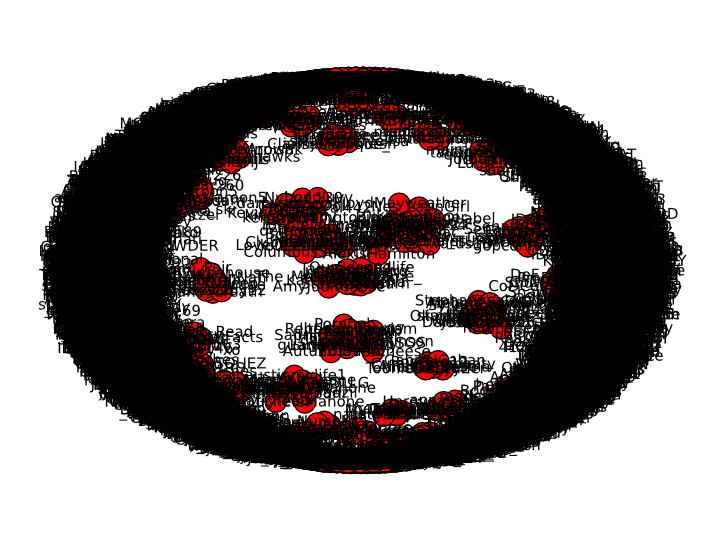
\includegraphics[scale=0.5]{./img/network.png}
    \caption{NetworkX Visualization of 10,000 retweets}
\end{figure}

\begin{figure}[ht]
    \centering
    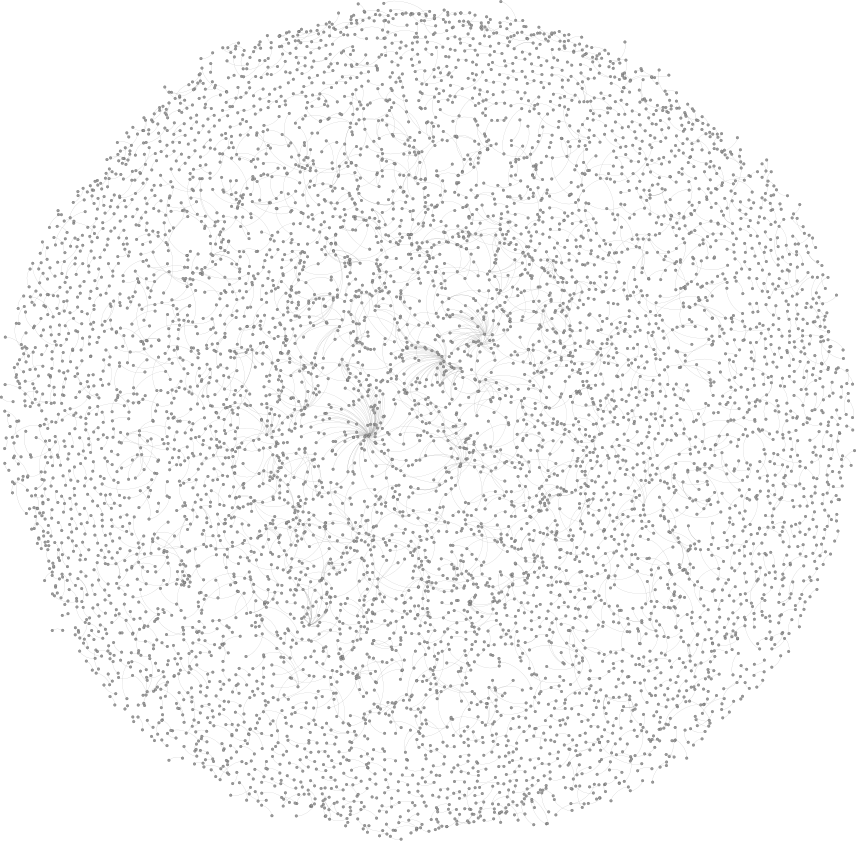
\includegraphics[scale=0.25]{./img/5000.png}
    \caption{Gephi Visualization of 5000 retweets}
\end{figure}

This network was created with a sample size of 10000 tweets. Each node that is visualized here is a retweet, and clusters appear when the individual that is retweeted is also in the sample. Conversely, the outer ring arises from the retweets that do not have a source tweet in the sample.

The relation to the class arises from the ranking system used. There are many different ways to implement a ranking system, many of which use a variety of matrices. A prime example of matrices that could be used are Markov Chains in order to determine probabilities in a manner similar to Google's PageRank. In order to correctly order these users, we can use the following fields:

    \begin{easylist}[enumerate]
        & \textbf{user[``id'']} - For uniquely identifying users.
        & \textbf{user[``screen\_name'']} - For uniquely identifying users in a readable format.
        & \textbf{user[``followers'']} - Number of followers the user has.
        & \textbf{user[``friends'']} - Number of friends the user has.
        & \textbf{text} - To identify retweets and possibly notable words/phrases.
    \end{easylist}

PageRank relies on the concept of an ``Anonymous Surfer'' who is randomly clicking links from page to page. This concept can be adapted to that of tweets and retweets, with each user acting as a ``page'', or a node, and each retweet or friend acting as a ``link'', or edge. This system relies on the eigenvalues of several matrices, and has high correlation with the material covered in this class.

The concept of ranking Twitter profiles on influence is interesting because Twitter holds a vast amount of information on our social lives, and by ranking individual users on their influence we can start to sift through Twitter feeds, identifying those that are the most important.

If we succeed in our endeavours, we will be able to not only sort through a set of twitter posts and rank the users on influence with respect to the others, we will also be able to take a given user profile and identify how influential the user is based on his twitter network and retweet percentages.

This project holds potential and can be adapted to a wide range of uses. It is also both accomplishable in the time allotted, and fits well into the scope of this course. We've been able to make enough preliminary progress as to determine that the dataset chosen is a good fit for this type of analysis. If completed well, we will be able to correctly rank users on their influence, a task that is not often thought of by Twitter users.

\end{document}
